\subsection{Thread Mapping}
With the control groundwork laid out in section~\ref{sec::stmImp}, its thread mapping and that of the simulation can be devised following the flowchart in Fig.~\ref{fig:controlFlowChart}.
 \lstinputlisting[language=C++, caption={Control Thread},label=lis:controlThread,style=customc]{./listing/controlThread.c}
Firstly the motors were configured (lines 6 through 13) with a callback that will update the measured linear velocity of each wheel (List.~\ref{lis:pcCallback}). Afterwards, the nine infrared odometric sensors were configured (lines 19 through 30), each sensor is configured with a callback (List.~\ref{lis:irsensorCallback}) that will update the distance to the nearest obstacle every update period, devised as 10 miliseconds in this instance. This callback checks the value read by the sensors and through a linear interpolation of the voltage/distance curve of the sensor, Fig.~\ref{fig:sensorCurvel}, the accurate distance in cm between the rover and the nearest obstacle can be measured. Next the streams for the communication between the navigation subsystem and the smartphone, along with the latter and the raspberry pi (lines 33 through 43), the callbacks in these streams (List.~\ref{lis:parseCallback}) are always updating the velocity and angle references, that should be altered whenever a command is received. Afterwards the navigation subsystem requests commands, fills an array with the distances for the obstacle avoidance algorithm to use and then makes use of the control algorithm established in section~\ref{sec::stmImp}.
 \lstinputlisting[language=C++, caption={Pc Callback},label=lis:pcCallback,style=customc]{./listing/pcCallback.c}
 \lstinputlisting[language=C++, caption={Ir Sensors Callback},label=lis:irsensorCallback,style=customc]{./listing/irsensorCallback.c}
 \lstinputlisting[language=C++, caption={Parse Callback},label=lis:parseCallback,style=customc]{./listing/parseCallback.c}

Afterwards the simulation thread merely makes use of the system model already used in the aforementioned section~\ref{sec::stmImp}.
 \lstinputlisting[language=C++, caption={Simulation Thread},label=lis:parseCallback,style=customc]{./listing/simulationThread.c}

Whenever the program needs to use global variables it makes use of a mutual exclusion object (mutex) that ensures that those variables cannot be shared simultaneously, ensuring a smooth and error avoiding execution.
\begin{figure}[!htbp]
\centering
       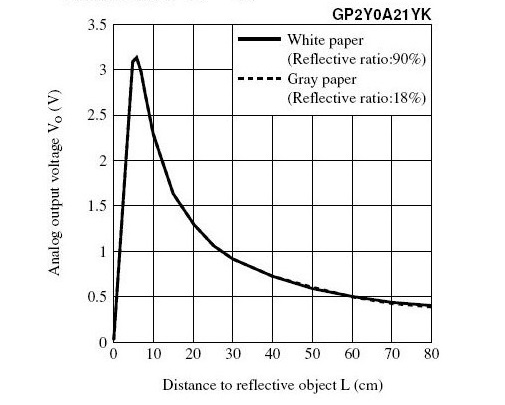
\includegraphics[page=1,width=0.6\textwidth]{img/sensorCurve.jpg} 
\caption{Voltage/Distance Curve of Sensor}%
\label{fig:sensorCurvel}
\end{figure}
\begin{figure}[!htbp]
\centering
       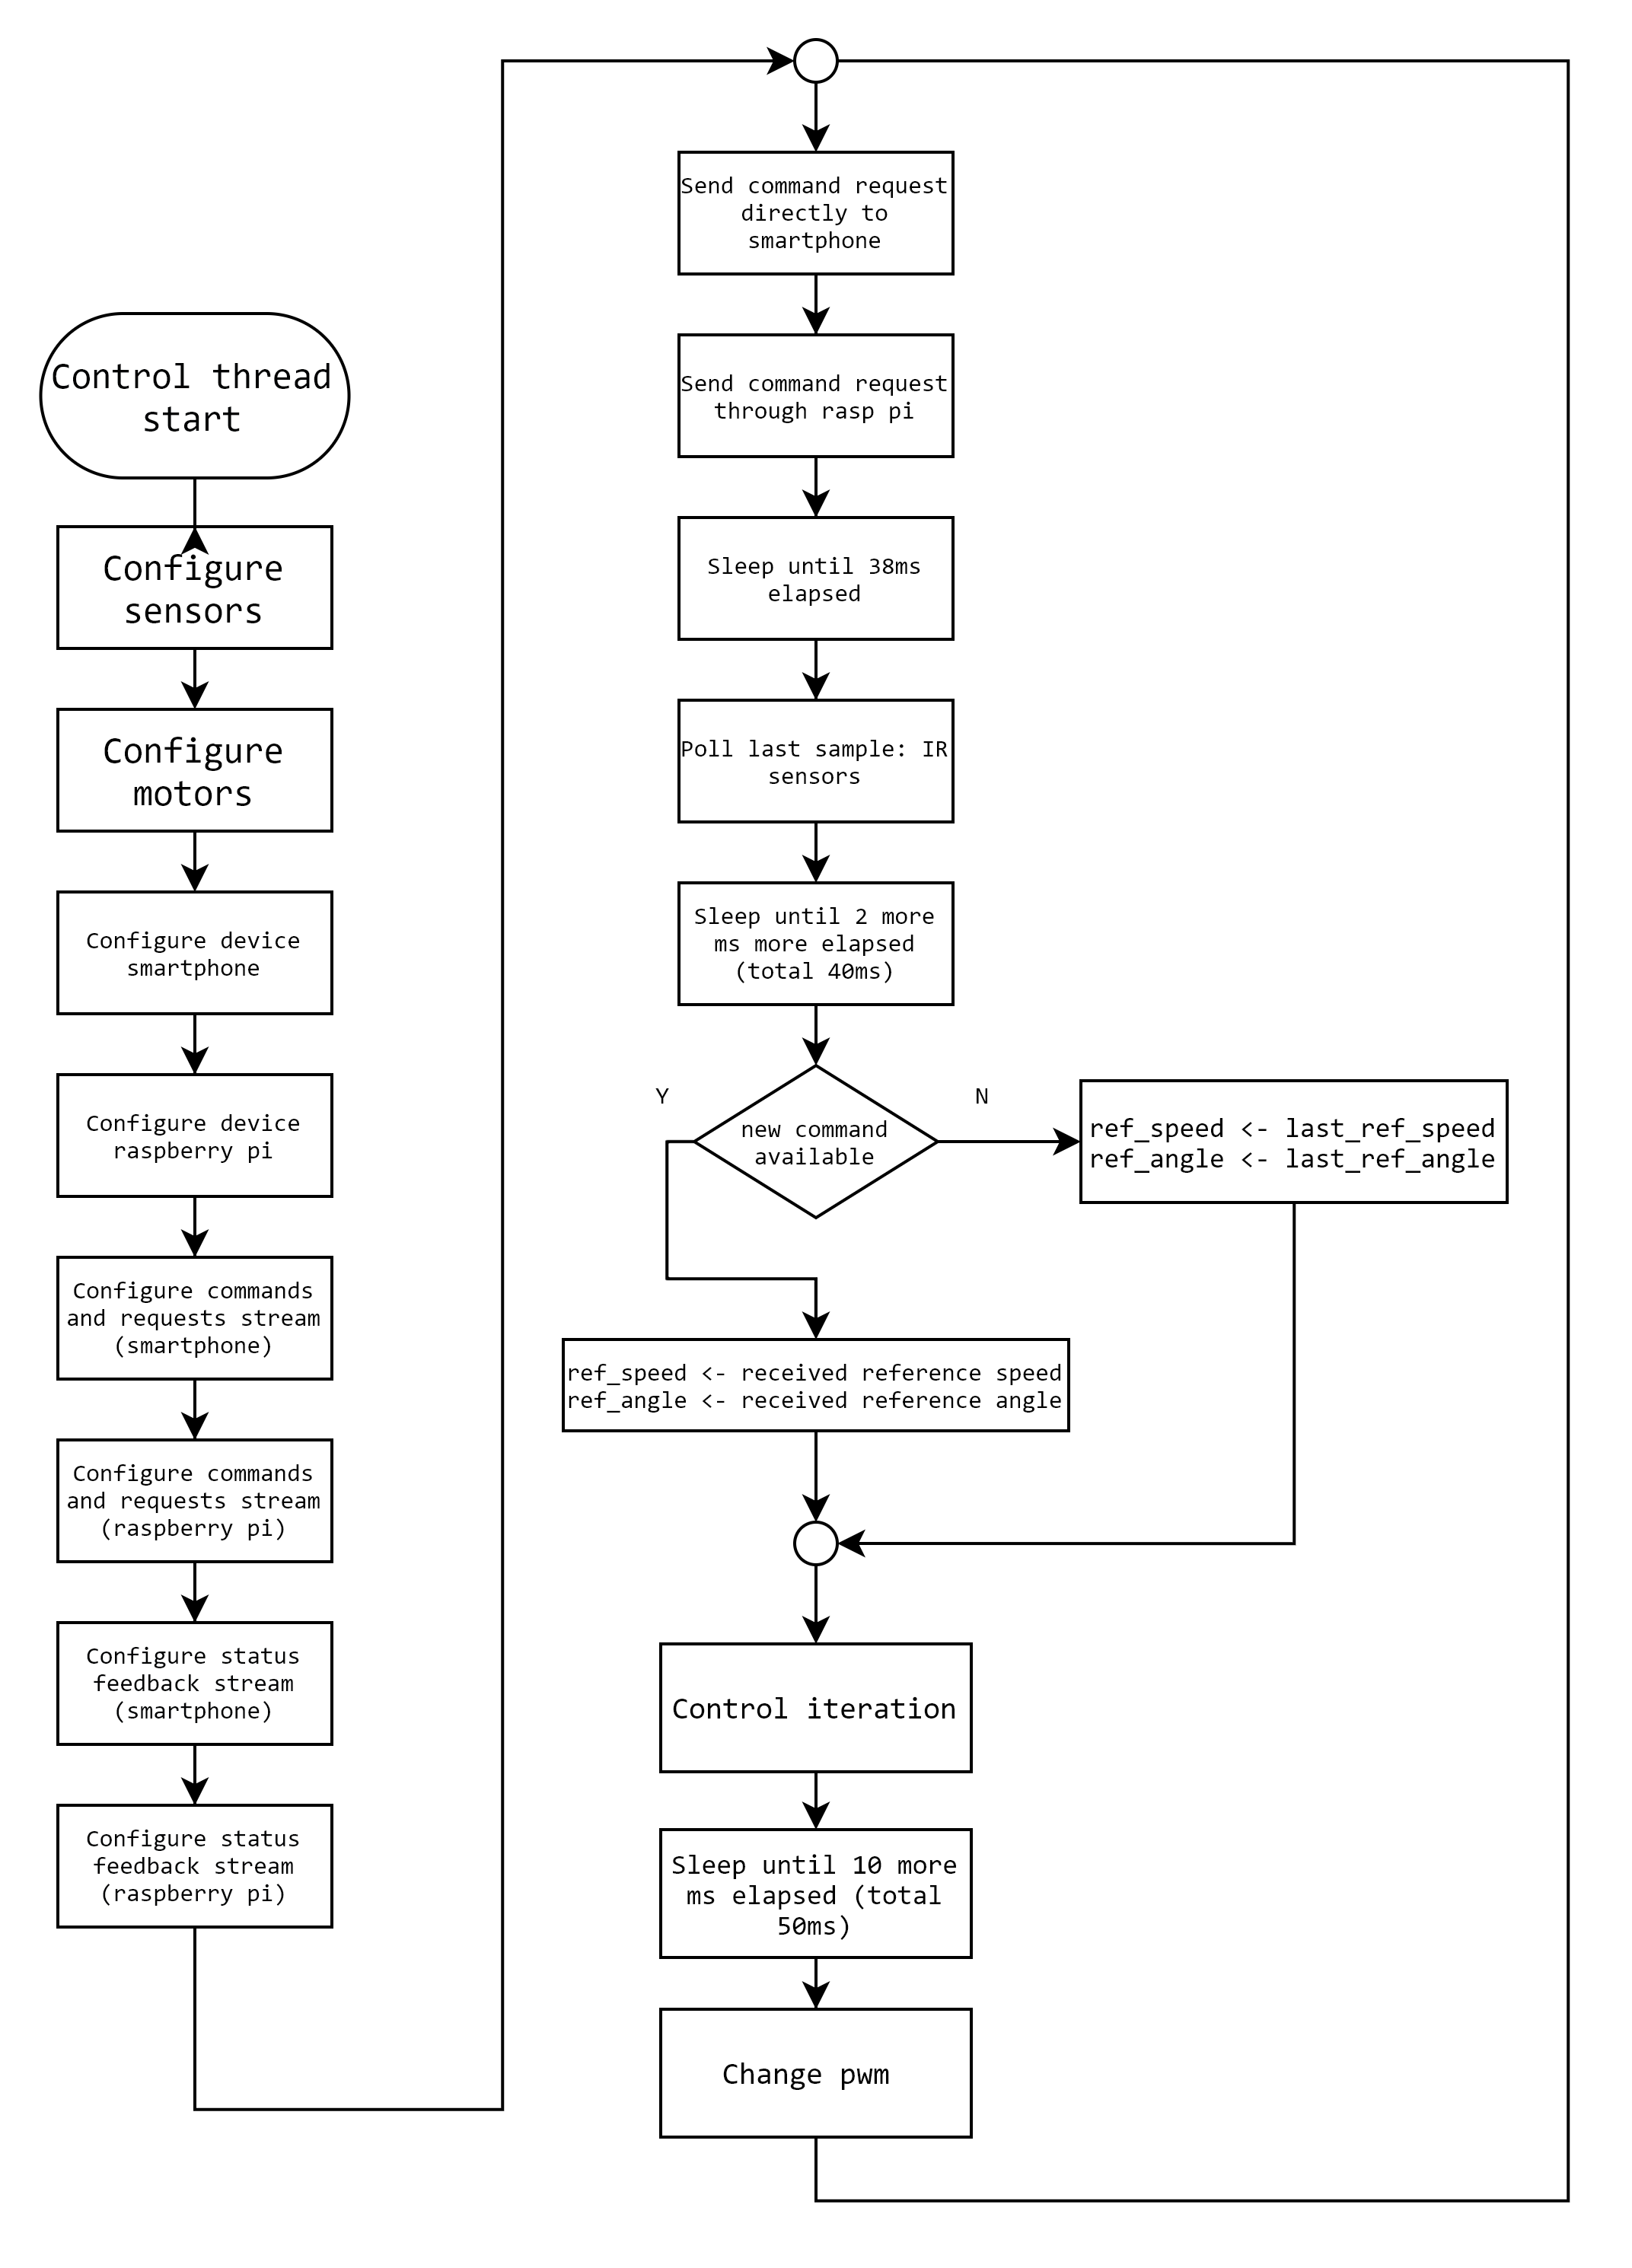
\includegraphics[page=1,width=0.8\textwidth]{img/controlThreadFlowchart.png} 
\caption{ControlThreadFlowchart}%
\label{fig:controlFlowChart}
\end{figure}